

\textbf{text gras}\hfill \\ \indent text indent�

%Ne pas mettre de caract�res accentu�s dans les titres ci-dessous
\chapter{chapX}\label{chapter:chapX}
\section{section}
\subsection{sous-section}
\subsubsection{sous-sous-section}


une ligne\\ une ligne � la ligne

\c{c} : �
\'{e} : �
\`{e} : �
\`{a} : �
\^{a} : �
\^{e} : �
\{
\%
\_
\textbackslash{}


\textquote{derri�re}


1\up{er}

%Juste une liste
\begin{itemize}
	\item un �l�ment de liste\index{ref pour l'index}
\end{itemize}
%
\begin{description}
	\item[un titre en gras] \hfill \\
	une description indent�e

\end{description}


\ref{figure:testProcess} page \pageref{figure:testProcess}

\begin{figure}[!h]% h || ht || .... cf 
  \centering
      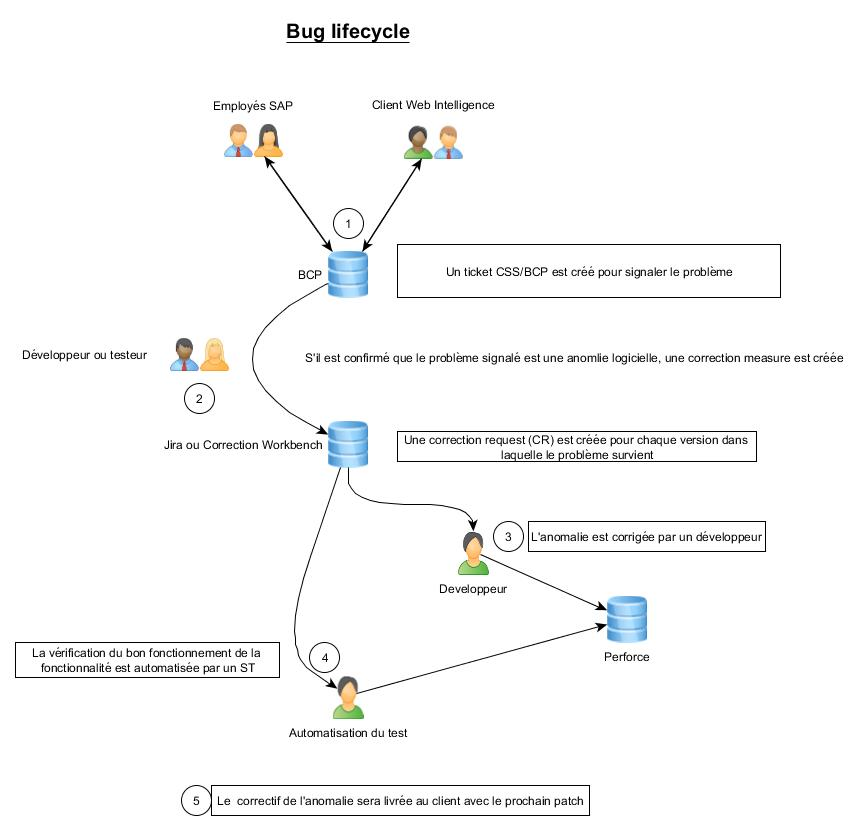
\includegraphics[width=\textwidth+1cm,height=\textheight-1.5cm]{images/testProcessAtSAP.jpg}
  \caption{Le process de test}
	\label{figure:testProcess}
\end{figure}


%Ins�rer du code
%Attention � la config n�cessaire !
\lstinputlisting[language=java]{scripts/basicStaticTest.java}


%plus simple mais verbeux
\begin{lstlisting}
MonoDocTestCase(MonoDocTestCaseConfigInfo tccInfo, String sDocumentName, String sCategoryType, String sCategory, Boolean useAuroraCtx);
\end{lstlisting}